%Preamble. You need all of this
%Document settings
\documentclass[letterpaper, 12pt]{article}
%Package for physics notation
\usepackage{physics}
%Package to display chemical equaltions
\usepackage{mhchem}
%proper typesetting of SI units
\usepackage{siunitx}
%Package to use other math symbols
\usepackage{amsthm}
%Set the margins as 1 inch because the default is 2.5 and looks bad
\usepackage[margin=1in]{geometry}
%Package for plotting data and making diagrams
\usepackage{pgfplots}
\usepackage{subfloat}
%Package to better customize figure placement
\usepackage{float}
%Package with more arrows (for plotting on axis)
\usetikzlibrary{arrows.meta}
%Package for Bra-Ket notation
\usepackage{braket}
%Package for more math notation
\usepackage{amsmath}
%Even more math notation
\usepackage{amssymb}
%Change line spacing to 1.45
\linespread{1.45}
\usepackage{import} %import documents so this tex file is short
\usepackage{lettrine} %i dont know what this does but I need it 
\usepackage{graphbox} %same
\usepackage{array}%Makes arrays which are more powerful tables
\usepackage{mathtools} %Lots of math tools
\usepackage{bm} %bold math font (for greek letters)
\usepackage{multirow} % for tables
\usepackage{cancel}
\usepackage{nomencl} %list of abbreveations
\renewcommand{\nomname}{List of Abbreviations}
\renewcommand{\nompreamble}{This list also provides brief descriptions of abbreviations which will be used throughout the body of the document}
%===========ABBREVEATIONS=================================
\makenomenclature

\nomenclature{CLO}{\textbf{Congruent localized orbital}; localized orbitals which reflect the symmetry of the molecular point group}

\nomenclature{HF}{\textbf{Hartree-Fock}; a fundamental electronic structure method in which $\Psi$ is represented by a single Slater determinant}

\nomenclature{MP$n$}{\textbf{$n$\textsuperscript{th} order M$\o$ller-Plesset perturbation}; a perturbative correction to HF approximation which adds correlation energy}

\nomenclature{CC}{\textbf{Coupled cluster}; size constituent post HF method which uses an exponential parametrization of H $e^{\hat{-T}}He^{\hat{T}}$}

\nomenclature{CCSD}{\textbf{CC singles and doubles}; CC method truncated at $\hat{T}_2$}

\nomenclature{CCSD(T)}{\textbf{CCSD with perturbative triples}; same as CCSD but contributions from triple excitations are estimated}

\nomenclature{EOM-CC}{\textbf{Equation-of-Motion CC}; extension of CC in which H is diagonalized over excited states}

\nomenclature{CI}{\textbf{Configuration interaction}; post HF method where $\Psi$ is expanded as a linear combination of excited states}

\nomenclature{MO}{\textbf{Molecular orbital}; orbitals built from a linear combination of atomic orbitals}

\nomenclature{AO}{\textbf{Atomic Orbital}; analytical one electron (hydrogen-like) functions}
\nomenclature{PNO}{\textbf{Pair natural orbital}; virtual orbitals assigned to electron pairs based on their spatial position}
\nomenclature{LPNO}{\textbf{Local PNO}; PNO implementation using localized orbitals (e.g., Foster-Boys}
\nomenclature{DLPNO-CC}{\textbf{Domain-based LPNO-CC}; LPNO implementation in which LPNOs are assigned to correlation domains in which they are highly localized}
\nomenclature{OSV}{\textbf{Orbital specific virtual}; Virtual orbitals assigned to specific electrons, (in contrast to PNO's which are assigned to election pairs)}
\nomenclature{FFT}{\textbf{Fast Fourier transform}; numerical method to calculate Fourier transforms of discrete data}


%=========================================================
%%%%%%%%%%NEW COMMANDS%%%%%%%

\newcommand{\adag}{a^{\dagger}} %Command for creation operator
%3 commands for matrix notation (pick one)
\newcommand{\matr}[1]{\bm{#1}} % undergraduate algebra version
%\newcommand{\matr}[1]{#1}          % pure math version
%\newcommand{\matr}[1]{\bm{#1}}     % ISO complying version
\newcommand{\secref[1]}{\S \ref{#1}}
%%%%%%%%%%%%%%%%%%%%%%%%%%%%%%
%%%%%%%%%Variable Declarations%%%%%%%%%%%%
\DeclareMathOperator\erfc{erfc}
%%%%%%%%%%%%%%%%
%%%%%%%%%%%%%%%% DOCUMET BEGINS HERE%%%%%%%%%%%%%%%%%%%%%%%%%%%%%%%%%
\begin{document}
\import{Sections/}{titlepage.tex} %ADD TITLE PAGE

\newpage %TITLE PAGE IS ITS OWN THING, NEW PAGE

\pagenumbering{roman} 
\setcounter{page}{2}
\section*{Abstract}
Recently, coupled cluster methods involving orbital localization have been shown to give highly accurate results while scaling like DFT. These localization methods are a massive step forward in the field of computational chemistry. Our aim is to utilize this localization and combine it with molecular symmetry to further speed up calculations on highly symmetric systems, in particular solids. We present the construction of \textit{congruent localized orbitals}, (CLOs), which are both localized and reflect the symmetry of the system. By using a CLO implementation of DLPNO-CC, we can exploit both sparsity and molecular symmetry, and eventually implement coupled cluster calculations in the solid state. In solid state systems, the long and short range interactions are partitioned, with the latter treated via Fourier transform. We wish to improve this partitioning by modifying the form of the long-range potential. 
\newpage
 %Change appendix numbering to i, ii, ...
\tableofcontents %Add toc
\listoffigures %add lof
\printnomenclature[3cm]

 

%%%%%%%%%%%%END OF ROMAN NUMBERED PAGES%%%%%%%%%%
\newpage 
\pagenumbering{arabic} %change page numbers back to 1, 2, 3...
\setcounter{page}{1} %Reset page counter so we don't mix roman numerals and numbers

%%%%%%%%%%%%%%%%%%%%%%%%%%%%%%%%%%%%%%%

%%%%%%%%%%%%%%%%%%%%%%%%%%%%%%%%%%%%%%%

\section{Introduction}
\subsection{Overview of the Problem}
Accurate calculations of chemical properties in the condensed state is an area of ongoing research in the field of computational chemistry. For weakly correlated materials, combinations of density functional theory and many-body pertubation theory have been shown to be give relativly accurate descripions of ground state properties \cite{solidCCSD}; however, as is the case with finite molecular systems, elucidation of excited state properties requires wavefunction based methods such as configuration interaction (CI) or coupled cluster (CC) singles and doubles (CCSD) with perturbative triples (CCSD(T)). It is plausable for such methods to use a combination of localized Gaussian orbitals and plane-waves as the basis of the calculation, combining the strengths of both bases. The small spatial extent of the localized Gaussian orbitals make them appropriate for treating short range interactions, while providing a compact basis for the virtual space. This basis may be used in a local treatment of electron correlation \cite{Booth}. Crystalline wavefunctions can be exactly expanded in an infinite plane-wave basis. This is a direct result of Bloch's theorem, which states that the wavefunction is congruent through lattice translations up to a global phase factor, 
\begin{align*}
\Psi_k(x+a)=e^{ika}\Psi_k(x)
\end{align*}
Where a is a lattice constant. A kinetic energy cutoff is chosen to limit the size of this axillary plane-wave basis.

Recently, McClain et. al. \cite{solidCCSD} presented the first excited-state CC treatment of diamond and silicon at the equation-of-motion CCSD (EOM-CCSD) level. After correcting for finite basis set effects, the band gaps were reported to be 5.37 \si{\eV} for diamond, compared to the experimental value of ~5.47 \si{\eV}, and 1.19 \si{\eV} for silicon, compared to an experimental value of 1.17 \si{\eV}. The main drawbacks of these methods are their computational complexity and memory usage. The complexity of periodic CCSD scales as $\mathcal{O}(n^2_{occ} n^4_{virt}N^4_k)$, while memory usage scales as $\mathcal{O}(n^2_{occ} n^2_{virt}N^3_k)$ where  $n_{occ}, n_{virt}$ are the number of occupied and virtual orbitals in the unit cell, and $N_k$ is the number of k-points \cite{solidCCSD}. The ground-state treatment of diamond was preformed using the TZVP basis and contained 256 electrons and 2176 orbitals, sampling 4x4x4 k-points in the Brillouin zone. This calculation took roughly 10,000 cpu hours, highlighting the harsh scaling of wavefunction based condensed matter methods. It is the goal of this research project to reduce this computational scaling via 
\begin{enumerate}
\item CLO based DLPNO-CCSD treatment of short-range interactions
\item Partitioning of Fock matrix contributions and t-amplitudes into short and long-range components
\end{enumerate} 
DLPNO-CCSD scales near-linearly for large finite systems while retaining chemical accuracy \cite{DLPNOCC}. Unlike the canonical orbitals, LPNOs are not constrained by the symmetry of the molecular point group. As a result, the complexity of LPNO calculations increases by a constant factor. While this increase is negligible for harshly scaling methods, it is significant for methods which scale near-linearly such as DLPNO-CCSD. By implementing CLOs in conjunction with DLPNO-CCSD, only symmetrically unique quantities will need to be calculated. Short-range contributions to t-amplitudes and the Fock matrix can be evaluated using this CLO DLPNO-CCSD while weaker long-range interactions may be treated perturbatively in Fourier space.

\subsection{Computational Methods}
\subsubsection{Hartree-Fock}
The Hartree-Fock (HF) method serves as a foundation for modern electronic structure techniques. The wavefunction, $\ket{\Psi}$, is taken to be a single determinant of a square matrix of one-electron functions, $\phi(x)$ \cite{HF}. For an n-electron system,
\begin{align}
\ket{\Psi}&= \frac{1}{\sqrt{N!}} \,
\begin{tabular}{|c c c c|}
$\phi_i(x_1)$ & $\phi_j(x_1)$& $\cdots$ & $\phi_n(x_1)$\\
$\phi_i(x_2)$ & $\phi_j(x_2)$&$\cdots$ & $\phi_n(x_2)$\\
$\vdots$ & $\vdots$& $\ddots$ & $\vdots$ \\
$\phi_i(x_n)$ & $\phi_j(x_n)$&$\cdots$  & $\phi_n(x_n)$\\
\end{tabular}
\end{align}
With the shorthand
\begin{align}
\ket{\Psi} &= \ket{\phi_i} \ket{\phi_j} \dots \ket{\phi_n} \\
&= \ket{\phi_i \phi_j \dots \phi_n} \\
&= \ket{ij \dots n} 
\end{align}
The ground state energy, $E_{HF}$, is given by the expectation value of the Hamiltonian, $\hat{H}$. In terms of one and two electron integrals, $E_{HF}$ can be written 
\begin{align}
E_{HF} &= \bra{\Psi} \hat{H} \ket{\Psi} \\ 
&=\overbrace{\sum_{i} \bra{i} h \ket{i}}^\text{1-e orbital energy} + \overbrace{\sum_{j>i} \braket{ij|ij}- \braket{ij|ji}}^\text{e-e repulsion and exchange} & i,j \in \text{occ. orbitals}
\end{align} 
Through HF, an approximate solution to the electronic Schr\"{o}dinger equation is easily attainable. If $\ket{\Psi}$ can be well modelled by a single determinant, HF is surprisingly accurate in absolute terms. The total electronic energy is accurate to 1\% of the true value \cite{Helgaker}. However, thermochemistry is governed by energy differences which are small relative to the overall energy. A one percent error often amounts to be several hundred \si{\kilo\joule\per\mol}.  Even in ideal cases, HF methods have a built-in error when describing many electron systems. This error stems from HF's lack of electron correlation interactions. HF treats each electron as interacting with an average field of the other electrons, when in reality the individual interactions between electrons are instantaneous and correlated. While these correlation effects are quite small in magnitude relative to the overall electronic energy, their energy differences are large with respect to what is considered acceptable error ($\leq$ 4 \si{\kilo\joule\per\mol}). Correlation effects must be included to make realistic chemical predictions 

\subsubsection{M$\o$ller-Plesset Perturbation Theory}
To improve the accuracy of a Hartree-Fock calculation, an $n$\textsuperscript{th} order M$\o$ller-Plesset (MP$n$) correction can be made. This perturbative correction to $E_{HF}$ approximates energy contributions from electron correlation. \cite{SO} Second-order M$\o$ller-Plesset (MP2) corrections are often utilized as they provide reasonable estimates of correlation energies with minimal impact on complexity. 
The Schr\"{o}dinger equation used in MP methods is
\begin{align}
\hat{H}\Psi&=(\hat{H}^0 +\lambda \hat{V}) \Psi=E\Psi &\lambda \in \mathbb{R}
\end{align} 
Where $\hat{V}$ is the correction to the unperturbed Hamiltonian, $\hat{H}^0$, and $\lambda$ is an arbitrary parameter which controls the strength of the perturbation. The n-th order terms are determined by expanding $\Psi$ and E in terms of powers of $\lambda$.
\begin{align}
(\hat{H}^0 + \hat{V}) \sum\limits_i^n \lambda^i \Psi^{(i)} &= \sum\limits_j^n \lambda^j E^{(j)} \sum\limits_k^n \lambda^k \Psi^{(k)}  
\end{align}
The zeroth order (uncorrected) energy is the energy of the unperturbed system, as expected. The first order correction to the energy ($E^{(1)}$) is given by
\begin{align}
\hat{H}^0 \ket{\Psi^{(1)}} + \hat{V}\ket{\Psi^{(0)}}&=E^{(0)}\ket{\Psi^{(1)}} + E^{(1)}\ket{\Psi^{(0)}}\\
\cancel{\bra{\Psi^{(0)}}\hat{H}^0 \ket{\Psi^{(1)}}} + \bra{\Psi^{(0)}}\hat{V}\ket{\Psi^{(0)}} &=\cancel{\bra{\Psi^{(0)}}E^{(0)}\ket{\Psi^{(1)}}} +\bra{\Psi^{(0)}} E^{(1)}\ket{\Psi^{(0)}}\\
\bra{\Psi^{(0)}}\hat{V}\ket{\Psi^{(0)}} &= E^{(1)} \braket{\Psi^{(0)} | \Psi^{(0)}}\\
E^{(1)} &= \bra{\Psi^{(0)}}\hat{V}\ket{\Psi^{(0)}} 
\end{align}
Which is the expectation value of the correction. The MP2 correction to the Hartree-Fock state is given by 
\begin{align}
E^{(2)} &= \frac{1}{4} \sum\limits_{i,j}^{N_{occ}} \sum\limits_{a,b}^{N_{virt}} \frac{|\braket{ab||ij}|^2}{\varepsilon_i + \varepsilon_j -\varepsilon_a-\varepsilon_b}
\end{align} 
Where $i,j$ refer to occupied orbitals, $a, b$ refer to virtual (unoccupied) orbitals, $\varepsilon_p$ is the energy of orbital p,  and $N_{occ}$, $N_{Virt}$ are the number of occupied and virtual orbitals, respectively.
\subsubsection{Coupled Cluster Theory}
The main drawback of single determinant methods such as HF is that the motions of anti-parallel spin electrons within the system are uncorrelated. For example, let $\ket{\Phi_{1s}}$ represent a doubly occupied 1s orbtal:

\begin{align}
\ket{\Phi_{1s}}&=\frac{1}{\sqrt{2}} \,
\begin{tabular}{|c c|}
$\phi_{1s}(x_1)$ & $\bar{\phi}_{1s}(x_1)$ \\
$\phi_{1s}(x_2)$ & $\bar{\phi}_{1s}(x_2)$\\
\end{tabular}
\end{align}

Where the bar denotes a spin-down orbital. It can be shown \cite{SO}
that once spin is integrated out, the probability of finding the two electrons at a point $(x_1,x_2)$ is \begin{align}
\mathcal{P}(x_1, x_2)= ||\phi_{1s}(x_1)||^2 \, ||\bar{\phi}_{1s}(x_2) ||^2
\end{align}
That is, if the two electrons have anti-parallel spin, the position of one electron does not depend on the other. Thus, the motion of these electrons are uncorrelated. To include these correlation effects, we will introduce a \textit{cluster function} $\mathcal{F}_{ij}$,  
\begin{align}
\mathcal{F}_{ij}(x_m, x_n) = \sum_{a>b} f^{ab}_{ij} \, \phi_a(x_m) \phi_b(x_n) 
\end{align}
Where the $f^{ab}_{ij}$ are coefficients which will be solved via the electronic  Schr\"{o}dinger equation. $\mathcal{F}_{ij}$ correlates the motions of two electrons within orbitals i,j \cite{reviews}. Adding this to a many electron single-determinant reference wavefunction, $\ket{\Phi_{0}}$, yields
\begin{align}
\ket{\Psi}&= \ket{\phi_i \phi_j... \phi_n} +
 \sum_{a>b} f^{ab}_{ij} \ket{\phi_a\phi_b ... \phi_n}\\
 &= \ket{\Phi_{0}} + \sum f^{ab}_{ij} \adag_a \adag_b a_j a_i\ket{\Phi_{0}} 
\end{align}
Where $a^\dagger_p$ creates an electron in orbital p, while $a_q$ removes an electron from orbital q. $a^\dagger_p$ and $a_q$ are denoted the creation and annihilation operators, respectively. For systems with many electrons, we can approximate the true wavefunction by expanding a reference HF wavefunction in a "basis" of cluster functions such that our approximation, $\ket{\Psi}$, includes correlation between n-tuples of electrons:
\begin{align}
\ket{\Psi}&=  \bigg(1 +\sum_{ai} f^a_i \adag_a a_i + \sum_{abij} f^{ab}_{ij} \adag_a \adag_b a_j a_i  +...\bigg) \ket{\Phi_{0}} \label{eq:cluster}
\end{align}

In examining \eqref{eq:cluster} we see that when electron correlation effects are included, $\ket{\Psi}$ becomes a linear combination of Slater determinants, where subsequent determinants are generated by replacing occupied orbitals in $\ket{\Phi_{0}}$ with virtual orbitals. This replacement is analogous to exciting an electron from an occupied orbital into the virtual space. To make the transition to conventional CC theory, we define total single, double, and n-th order excitation operators, $\hat{T}_1$, $\hat{T}_2$, and $\hat{T}_n$, respectively, in terms of our original $f$ coefficients (henceforth referred to as t-amplitudes): \begin{align}
\hat{T}_1 &\equiv \sum_{i}  \hat{t}_i = \sum_{ia}  t^a_i \adag_a a_i\\
\hat{T}_2 &\equiv \frac{1}{2} \sum_{ij}  \hat{t}_{ij}  = \frac{1}{4}\sum_{ijab}  f^{ab}_{ij}\adag_a \adag_b a_j a_i \\
\hat{T}_n &\equiv \bigg(\frac{1}{n!}\bigg)^2 \sum_{ij\dots ab\dots} f^{ab\dots}_{ij\dots} 
\end{align}
As well as the total cluster operator, $\hat{T}$
\begin{align}
\hat{T} &\equiv \hat{T}_1 + \hat{T}_2 + \dots \hat{T}_n
\end{align}

The CC approximation of the true wavefunciton is defined by an exponential parametrization using the Taylor expansion of $e^x$. Equation \eqref{eq:ansatz} is known as the exponential ansatz, a central equation in CC theory.

\begin{align}
\ket{\Psi} \label{eq:ansatz}&= e^{\hat{T}} \ket{\Phi_{0}} =e^{\hat{T}_1 + \hat{T}_2 + ... }  \ket{\Phi_{0}}\\ 
&= \sum_n \frac{\big(\hat{T}_1 + \hat{T}_2 + ...  \big)^n}{n!} \ket{\Phi_{0}}\\
 &=  \bigg(1 + \hat{T}_1 + \hat{T}_2 + \frac{1}{2!} \hat{T}^2_1 +  \hat{T}_2\hat{T}_1 + \frac{1}{2!}\hat{T}^2_2 \bigg)\ket{\Phi_{0}}\\
&= \bigg(1 +
\underbrace{\sum_{i} \hat{t}_i}_{\hat{T}_1} +
\underbrace{\frac{1}{2} \sum_{i,j} \hat{t}_{ij}}_{\hat{T}_2} +
\underbrace{\frac{1}{2} \sum_{i,j} \hat{t_i} \hat{t_j}}_{\frac{1}{2}\hat{T}^2_1}  + 
\underbrace{\frac{1}{2} \sum_{i,j}\sum_{k} \hat{t}_{ij}\hat{t}_{k}}_{\hat{T}_2 \hat{T}_1} + ... \bigg) \ket{\Phi_{0}} \label{eq:ansatzExpansion}
\end{align} 


Coupled-cluster methods have the crucial benefit of being size-consistent at any level of truncation. That is, for two non-interacting molecules A and B, the overall energy of the system is equal to the sum of the individual molecular energies:
\begin{equation}
E_{AB}= E_{A} + E_{B}
\end{equation}
The size consistency of both full and truncated CC methods is due to the exponential ansatz, as the exponential (and the reference wavefunction) may be separated into products of single-molecule components:
\begin{equation}
\Psi_{cc}=e^{\hat{T}} \ket{\Phi_0} = e^{\hat{T}_A + \hat{T}_B}\ket{\Phi_0} = e^{\hat{T}_A} e^{\hat{T}_B}\ket{\Phi_0}
\end{equation}
This is in direct contrast to CI methods, in which the CI wavefunction is written in an expansion of $\hat{C}$ excitation operators:
\begin{equation}
\Psi_{CI} = (1 + \hat{C}) \ket{\Phi_0} =  (1 + \hat{C}^A + \hat{C}^B)\ket{\Phi_0}
\end{equation}
Consider a system of two non-interacting \ce{H2} molecules, denoted (\ce{H2})$^A$ and (\ce{H2})$^B$. In the case of using truncated CI singles and doubles (CISD), the wavefunction takes the form 
\begin{equation}
\Psi_{CISD} = (1+\hat{C}) \ket{\Phi_0}=(1+\hat{C}_1+\hat{C}_2) \ket{\Phi_0}
\end{equation}
Thus the \textit{overall} system is restricted to double excitations. Configurations in which \textit{either} (\ce{H2})$^A$ or (\ce{H2})$^B$ is doubly excited is represented in the CISD wavefunction, but the configuration in which \textit{both} (\ce{H2})$^A$ \textit{and} (\ce{H2})$^B$ are doubly excited is excluded, because that configuration would be analogous to a quadruple excitation for the overall system. \cite{SO}
On the other hand, expansion of the exponential ansatz in CCSD gives higher-order excitations through products of excitation operators. For example, the final written term in \eqref{eq:ansatzExpansion}, $\hat{T}_2\hat{T}_1$, is equivalent to an overall triple excitation, and terms such as $\hat{T}_2 (\hat{T}_1)^2$ and $(\hat{T}_2)^2$ are overall quadruple excitations. \\


An expression for the CC energy is obtained by substituting \eqref{eq:ansatz} into the Schr\"{o}dinger equation, 
\begin{align}
\hat{H} e^{\hat{T}}\ket{\Phi_{0}} &=  e^{\hat{T}} E \ket{\Phi_{0}}\\
e^{-\hat{T}} \hat{H} e^{\hat{T}}\ket{\Phi_{0}} &=E\ket{\Phi_{0}}\label{eq:ansatz schroginger}
\end{align}
By left-projecting excited determinants generated by $\hat{T}$  onto \eqref{eq:ansatz schroginger}, a system of non-linear equations is generated: 
\begin{align}
\begin{split}
\braket{\Phi^a_{i}| e^{-\hat{T}} \hat{H} e^{\hat{T}} |\Phi_{0}} &= 0 \\
\braket{\Phi^{ab}_{ij}| e^{-\hat{T}} \hat{H} e^{\hat{T}} |\Phi_{0}} &= 0\\ 
\vdots\\
\braket{\Phi^{a\dots}_{i\dots}| e^{-\hat{T}} \hat{H} e^{\hat{T}}|\Phi_{0}} &=0
\end{split}
\end{align}
Where, for example, projection by $\bra{\Phi^{a}_i}$ generates an expression which couples $t^a_i$ to the energy and other t-amplitudes. Once these equations are solved and the t-amplitudes are known, the energy is readily available, and can be written analytically as  
\begin{equation}
\braket{\Phi_0 | \hat{H} | \Phi_0} + \braket{\Phi_0 | \hat{H}  \hat{T}| \Phi_0} + \braket{\Phi_0 | \hat{H} \frac{\hat{T}^2}{2}| \Phi_0} = E
\end{equation}
This equation is correct regardless of where $\hat{T}$ is truncated \cite{reviews}.  \\

Energy contributions from higher order excitations are small in magnitude; thus, it is often sufficient to truncate $\hat{T}$ at a specific $\hat{T_n}$. Higher-order excitations can then be ignored, or approximated with a perturbative method analogous to MP2. CCSD and CCSDT truncate $\hat{T_n}$ to include double and triple excitations, respectively, while CCSD(T), the 'gold-standard' of quantum chemistry, approximates triple excitations using perturbation theory. The CC methods are able to accurately determine reaction energies, NMR shifts, and other difficult to predict properties. The main drawback of CC methods is their harsh scaling; CCSD, CCSD(T), and CCSDT, scale as $\mathcal{O}(N^6)$, $\mathcal{O}(N^7)$, and $\mathcal{O}(N^8)$, respectively. Techniques to speed up computational methods are at the heart of computational chemistry and will be discussed throughout \S\ref{Efficient Electronic Structure}
\subsection{Efficient Electronic Structure} \label{Efficient Electronic Structure}
\subsubsection{Molecular Symmetry}

Electronic structure calculations are performed at a fixed molecular geometry, and thus it is useful to define orbitals that transform in a well defined fashion with the Hamiltonian, based on the geometry of the system. Molecules are classified by their \textit{point-group}, $\mathcal{G}$; a set of symmetry operations under which the molecule remains unchanged. In the case of finite molecular systems, the symmetric operations include the identity ($\hat{E}$), $\frac{2\pi}{n}$ rotations ($\hat{C_n}$), reflections ($\hat{\sigma}$), and inversions ($\hat{i}$). Improper rotations ($\hat{S}_n \equiv \hat{C}_n \cdot \hat{\sigma} \mid \hat{\sigma} \bot \hat{C}_n$),  are defined for group closure \cite{Abstract}. As an example, the molecular point group of benzene is D$_{6h}$, and therefore any combination of symmetry operations in the D$_{6h}$ character table (e.g., $\hat{C}_6$) leave the molecule in a symmetrically equivalent orientation. The canonical molecular orbitals (MOs) then transform as irreducible representations ($\Gamma_i$'s) of the molecular point group, generated by block-diagonalizing a matrix representation of the group \cite{212}. The benzene $\pi$ system is comprised of four irreducible representations, $\Gamma_{\pi} = \Gamma_{A_{2u}} + \Gamma_{E_{1g}} + \Gamma_{E_{2u}} + \Gamma_{B_{2g}}$.

\begin{figure}[H]
	\centering
	\begin{tabular}[m]{m{0.2\textwidth} m{0.2\textwidth}m{0.2\textwidth}p{0.2\textwidth}}
		\multirow{2}*{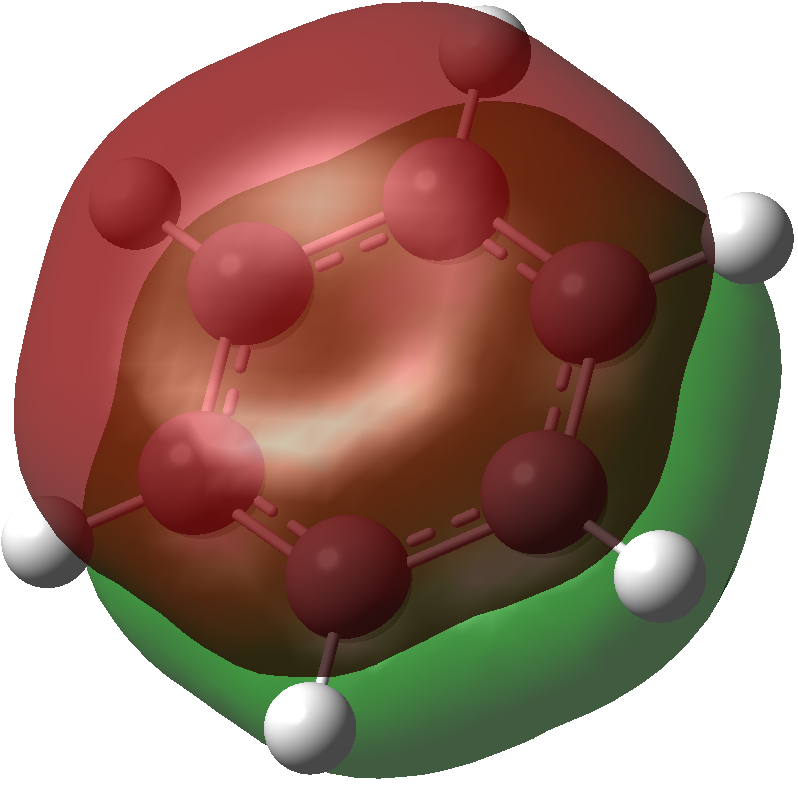
\includegraphics[width=0.15\textwidth]{Images/BenA2u.png}} 
	 	&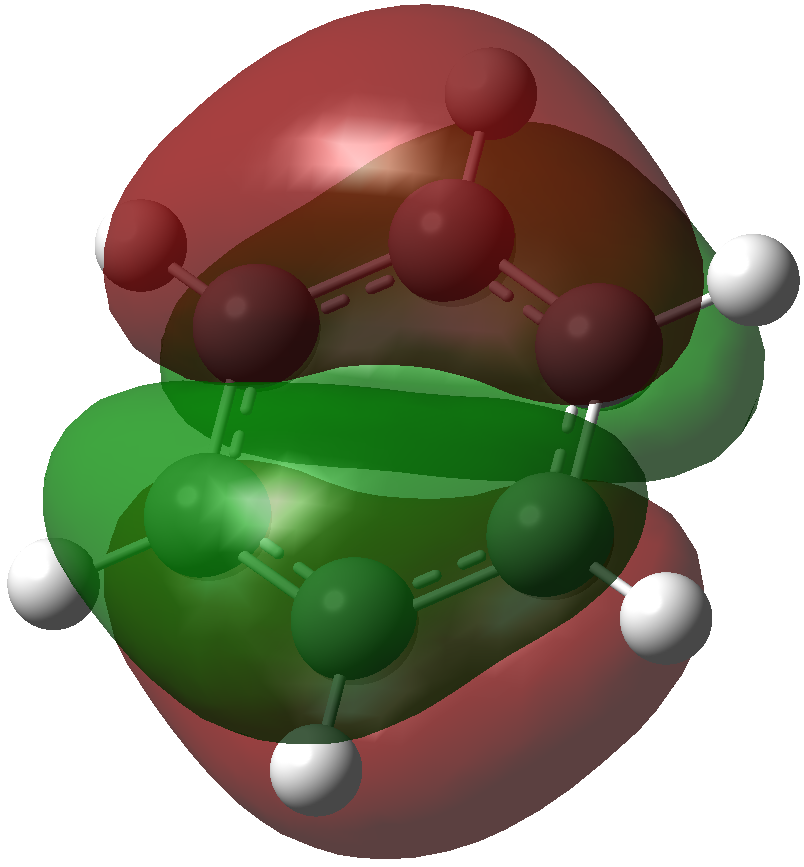
\includegraphics[width=0.15\textwidth]{Images/BenE1g1.png}
	 	&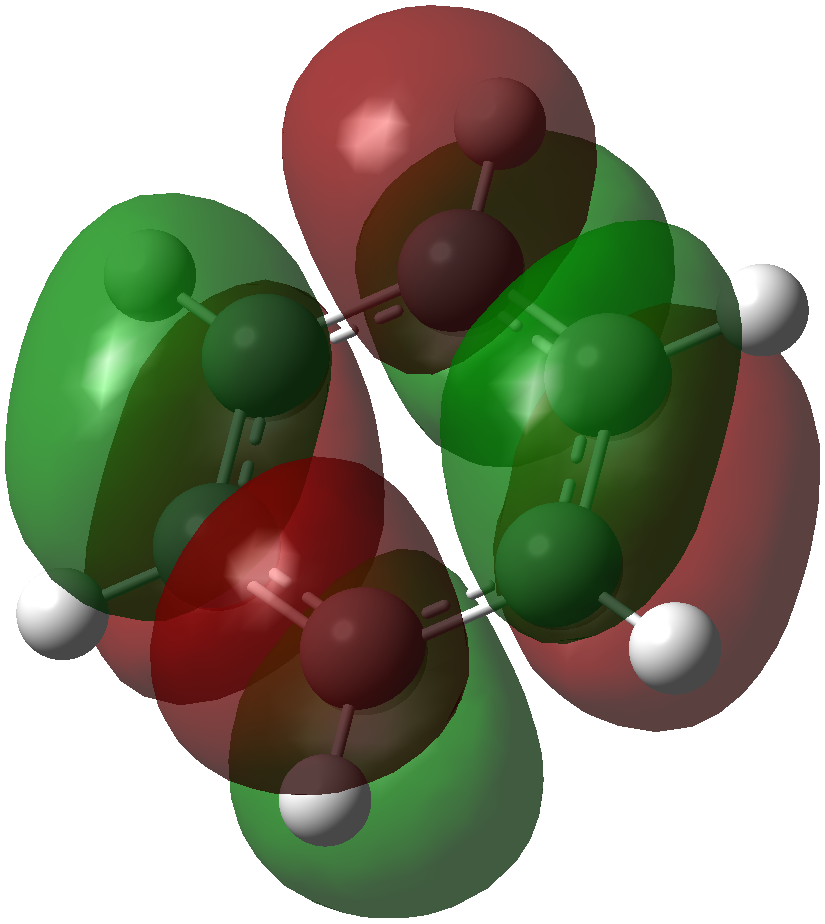
\includegraphics[width=0.15\textwidth]{Images/BenE2u1.png}
	 	&\multirow{2}*{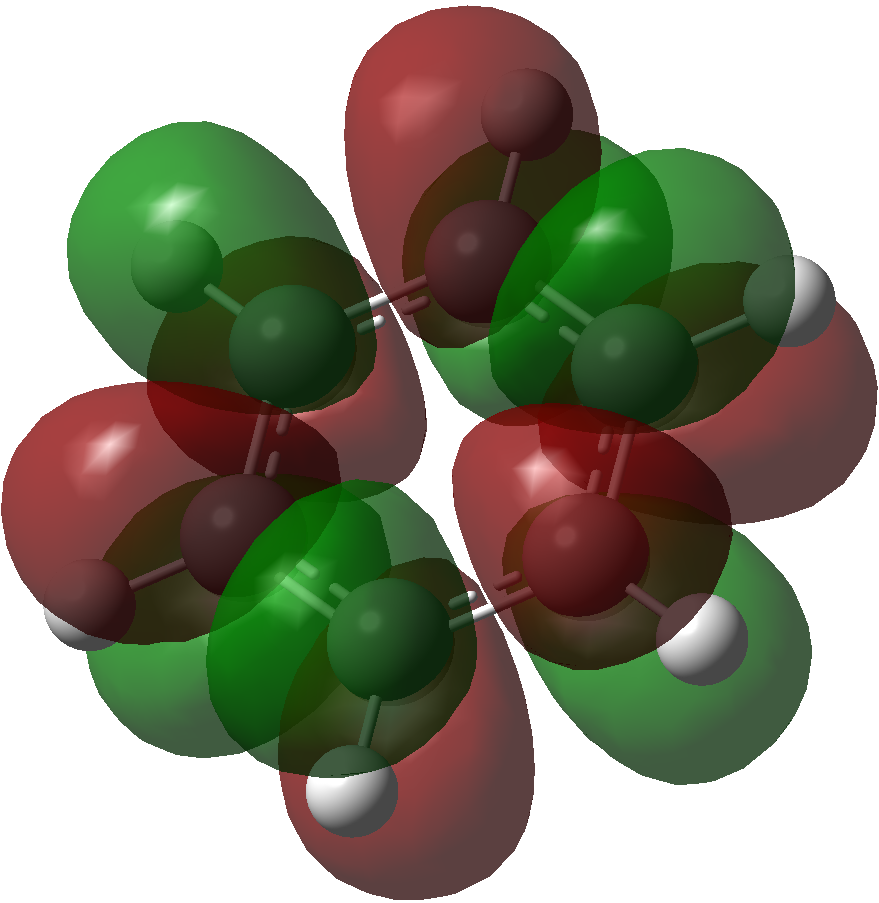
\includegraphics[width=0.15\textwidth]{Images/BenB2g.png}} \\
		&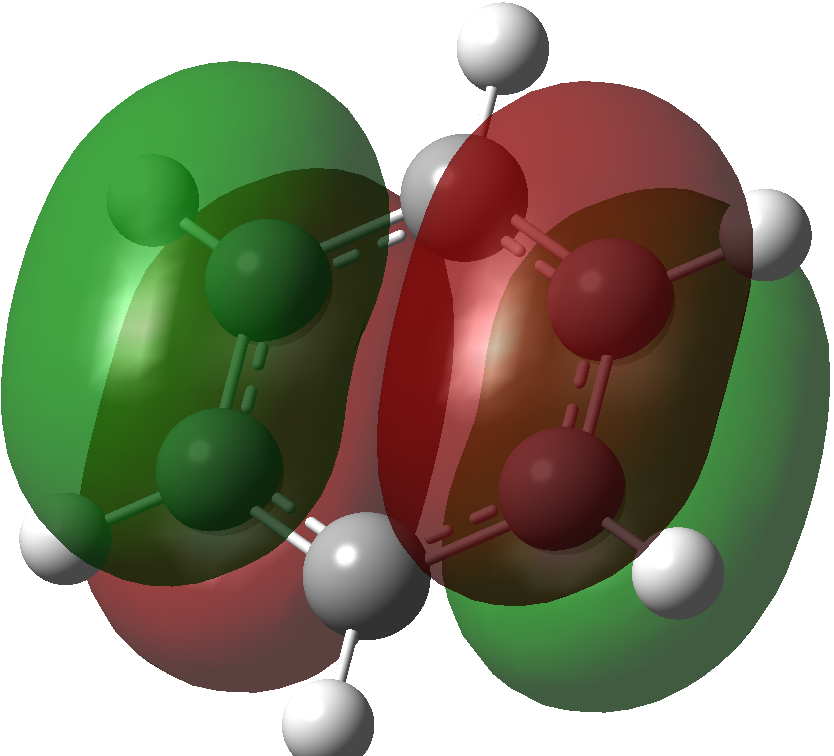
\includegraphics[width=0.15\textwidth]{Images/BenE1g2.png}
		&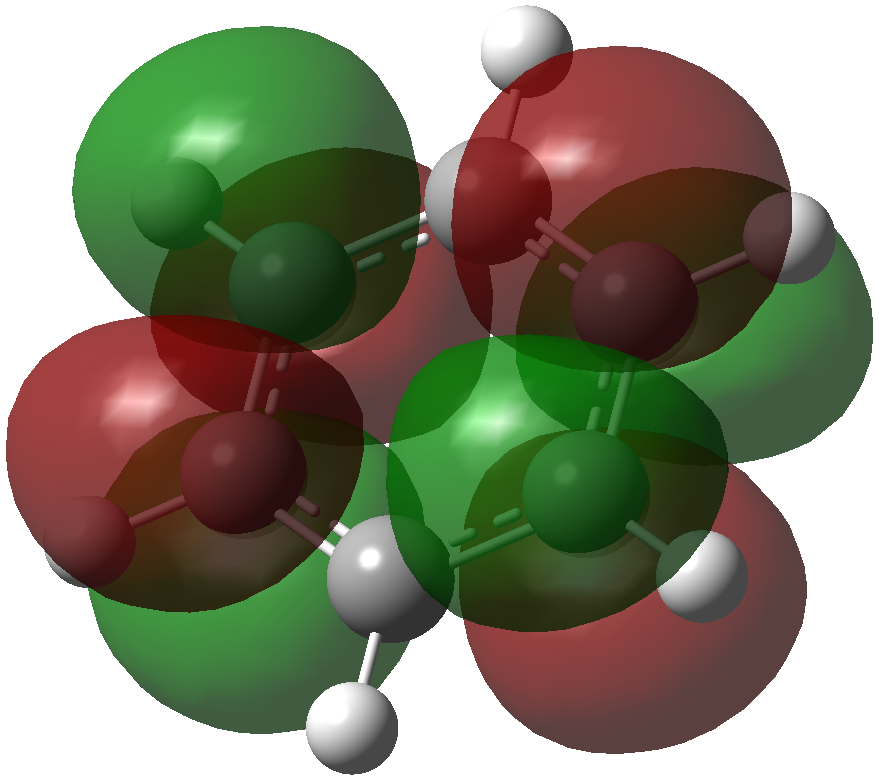
\includegraphics[width=0.15\textwidth]{Images/BenE2u2.png}\\
	
		\centering $A_{2u}$ &
		\centering $E_{1g}$ &
		\centering  $E_{2u}$ &
		\centering $B_{2g}$  \\
	\end{tabular}

	\caption{Canonical $\pi$ orbitals of benzene}
\label{fig:pirep}
\end{figure}
As can be seen in Figure \ref{fig:pirep}, the $\Gamma_E$'s are doubly degenerate. In general, any $\Gamma$ with degree $d \geq 2$ generates d degenerate MOs. Abelian groups such as $C_{2V}$ are comprised solely of one dimensional $\Gamma's$ and therefore molecules with $C_{2V}$ symmetry typically have no degenerate molecular orbitals. Mathematically, the electronic wavefunction transforms with respect to symmetry operations in $\mathcal{G}$ as described by it's irreducible representation. For non-degenerate states, this can be written:
\begin{align}
 \Psi(\{\mathcal{R}\}, \hat{R_i}x)&=e^{i\theta_i}\Psi(\{\mathcal{R}\},x), &\hat{R}_i \in \mathcal{G}
\end{align}
For some fixed geometry, $\{\mathcal{R}\}$ and symmetry operation, $\hat{R_i}$, the wavefunction is equal up to a global phase factor,  $e^{i\theta_i}$.
This can be extended into systems of solids which have translational symmetry; Siloxane polymers can be broken up into \ce{SiR2O} unit cells translated along the plane of the \ce{SiO} chain. Symmetry adapted orbitals then take the form of Bloch functions delocalized over the lattice:
\begin{equation}
\Psi_k(\{\mathcal{R}\},(x+a)) = e^{ika}\Psi_k(\{\mathcal{R}\},x) 
\end{equation}

Molecular symmetry places useful constraints on electron integrals and t-amplitudes. A given t-amplitude $t^{ab\dots}_{ij\dots}$, is zero unless the product of its irreducible representations contains the totally symmetric irreducible representation, $A_1$.
\begin{align}
\Gamma_a \otimes \Gamma_b \otimes \cdots \Gamma_i \otimes \Gamma_j \otimes \cdots  = A_1
\end{align}
This is because the action of $\hat{t}_{ij\dots}$ (an electronic excitation) does not change the symmetry of the reference wavefunction, 
\begin{align}
\Gamma_{\hat{t}_{ij\dots}} \otimes \Gamma_\Psi &= \Gamma_\Psi 
\end{align}
Which is only possible if $t_{ij\dots}$ contains $A_1$.

CC implementations make use of this by organizing MOs into blocks of symmetry, where only products of orbitals in the same symmetric block are considered. This gives our matrix of t-amplitudes, ${\matr{T}}$, a block diagonal form:
\begin{equation*}
\hat{T}_{n}=\begin{array}{c| c c c c c}
&A_1 & \Gamma_2 & \cdots & \Gamma_n\\
\hline
A_1 & X_{11} &0 & \cdots & 0\\
\Gamma_2  & 0 & X_{22} &\cdots&0\\
\vdots & \vdots &\vdots & \ddots & 0\\
\Gamma_n & 0&0 & \cdots & X_{nn}
\end{array}\label{eq:diag}
\end{equation*}
Where $X_{ii}$ is a non-zero sub-matrix. This partitioning reduces the computational computational cost by a constant factor of $h^2$, where h is the number of irreducible representations in a point group (e.g., $8^2=64$ for ethylene). While the speed gained from exploiting molecular symmetry is indeed significant, it is overshadowed by the $\mathcal{O}(N^7)$ complexity of CCSD(T) for large systems. To further reduce this computational complexity, we look to orbital localization. 
\subsubsection{Orbital Localization and DLPNO-CC}
The harsh scaling of CC methods largely stems from the delocalized character of the canonical basis orbitals \cite{DLPNOCC,MP2}. As electrons are added to the system, the number of correlated electron pairs increases quadratically, and in-turn the number of t-amplitudes increases as $N^4$. While electron correlation increases the complexity by at least $\mathcal{O}(N^4)$, the interaction falls with $r^{-6}$. To exploit this property, orbitals which are spatially localized are used. The major breakthrough in local correlation techniques was made recently when the idea of pair natural orbitals (PNOs), originally introduced by Meyer in 1973, was revived as an idealized basis for local electron correlation. \cite{MEYER, LPNOCC}. Techniques using localized PNOs were shown to be applicable to systems containing about 100 atoms. The key idea of PNOs is that a small set of virtual orbitals is associated with each specific pair of occupied orbitals.\\

The latest refinement described by Riplinger and Neese in 2013 assigns each PNO to a correlation domain in which it is highly localized. The result is a near linearly scaling domain-based local pair natural orbital implementation of CCSD, abbreviated DLPNO-CCSD \cite{DLPNOCC}. A set of localized orbitals, $\ket{i_L}$, is first generated via Foster-Boys localization, in which the spatial extent of the orbitals, $\braket{\hat{L}} = |\hat{r}_1 - \hat{r}_2|^2$, is minimized. A set of linearly dependent orbitals which span the active space, $\ket{\tilde{\mu}}$, are defined via projection of the atomic orbitals, $\ket{\mu}$, onto this localized basis:
\begin{align}
\ket{\tilde{\mu}} &= (1-\hat{P}) \ket{\mu}, &\hat{P} &= \sum_{i_L} \ket{i_L} \bra{i_L}
\end{align} 
Each orbital is then assigned to a correlation domain $\{A\}_i$ based on its spatial extent. Each domain typically consists of 10-30 atoms. The correlation energy ($\varepsilon^{OSV}_{ij}$) of each electron pair is then estimated via a linearly scaling pre-screening algorithm based on orbital specific virtuals (OSV). Electron pairs are then given different levels of treatment based on the magnitude of $\varepsilon^{OSV}_{ij}$:
\begin{itemize}
\item $\varepsilon^{OSV}_{ij} < 10^{-6}$ E$_h$, $\varepsilon^{OSV}_{ij}$ is taken to be the correlation energy
\item $\varepsilon^{OSV}_{ij} > 10^{-6}$ E$_h$, the pair is treated with MP2 $\rightarrow \varepsilon^{MP2}_{ij} $
\item $\varepsilon^{MP2}_{ij} > 10 ^{-4}$ E$_h$, the pair is given full CC treatment.
\end{itemize} 
This accuracy hierarchy reduces the number of t-amplitudes to be calculated by a factor of roughly $10^5$ for large systems, while retaining $> 99.5\%$ of the correlation energy \cite{DLPNOCC}. The result is that large molecular systems can be assessed at the CCSD level on a single core in a reasonable amount of time. In their paper describing DLPNO-CCSD, Riplinger and Neese reported two of the largest completed CCSD calculations at the time of publication: Vancomycin (Figure \ref{vanco}), a pharmaceutical used for antibiotic resistant-bacteria, and \ce{C150H302}, a polyethylene chain. The calculations were done via DLPNO-CCSD in the def2-TZVP basis and took 5 and 13 days to complete on a single core, respectively. CCSD treatment of such massive molecules was previously unheard of. In both cases, less than 10\% of all electron pairs were given full cc treatment (9.4\% for vancomycin and 4\% for \ce{C150H302}). This results in a massive computational speed-up. In large systems, the DLPNO-CCSD calculation completed faster than the preceding HF calculation.
It is clear that DLPNO-CC produces results on par with non-localized CC methods, while completely defeating them in terms of computational efficiency. 
\begin{figure}
\centering
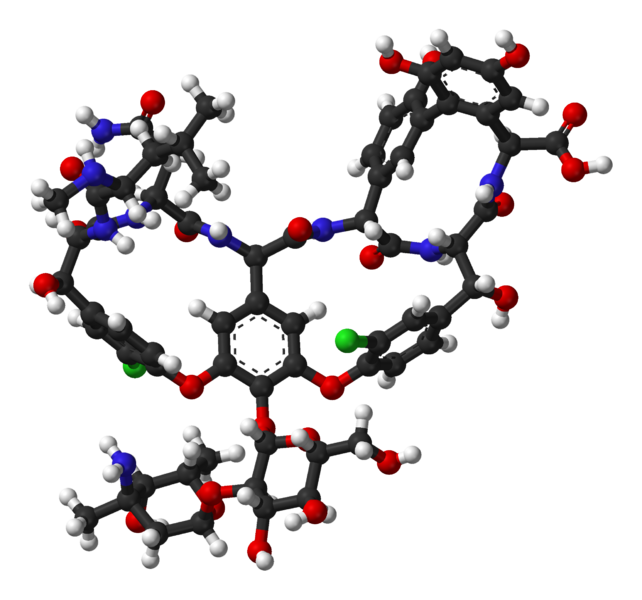
\includegraphics[scale=0.35]{Images/Vanco.png}
\caption{Chemical structure of vancomycin: 176 atoms, 3593 basis functions using the def2-TZVP basis}
\label{vanco}
\end{figure}

\subsubsection{Congruent Localized Orbitals}
Just as solids can be broken up into a unit cell which is periodic through a lattice translation, finite molecules can be broken up into unit-cells which are congruent through transformations in the molecular point group. Benzene, for example, can be thought of as a \ce{CH} 'unit cell' which is congruent through transformations in $\{C_{6}\}$ (Figure \ref{Fig:unit cell}). As with solids, individual unit cells are indistinguishable, thus it is not unreasonable to assume we can find a set of molecular orbitals which:
\begin{enumerate}
\item Are localized onto the unit cell
\item Are congruent through operations in a subgroup, $\mathcal{H}$, of the full molecular point group (space group), $\mathcal{G}$
\end{enumerate}
Localized orbitals such as the modified Foster-Boys orbitals used in DLPNO-CC fail to meet this criteria because the number of localized orbitals is always the same as the number of occupied orbitals. In the case of benzene, there are three occupied $\pi$-orbitals. However a benzene molecule is comprised of six unit cells, so at least six localized $\pi$ orbitals are needed. For localized orbitals to fully exploit molecular symmetry, this restraint must be lifted.  We define \textit{congruent localized orbitals} (CLOs) who's construction is discussed in detail in \S \ref{subsec:ConstructionCLO}. Some example CLOs were constructed in ACESII in the 3-21G basis and plotted in MOLDEN. Images of the benzene $\pi$ ClOs and \ce{CC} $\sigma$ bonding CLOs are shown in Figures \ref{fig:PiClo} and \ref{fig:SigClo}, respectively. \\

\begin{figure}
	\begin{tabular}[m]{m{6.5cm}m{1cm}m{7.5cm}}
	{
		\begin{tabular}[m]{m{3cm} m{.75cm} m{3cm}}
			{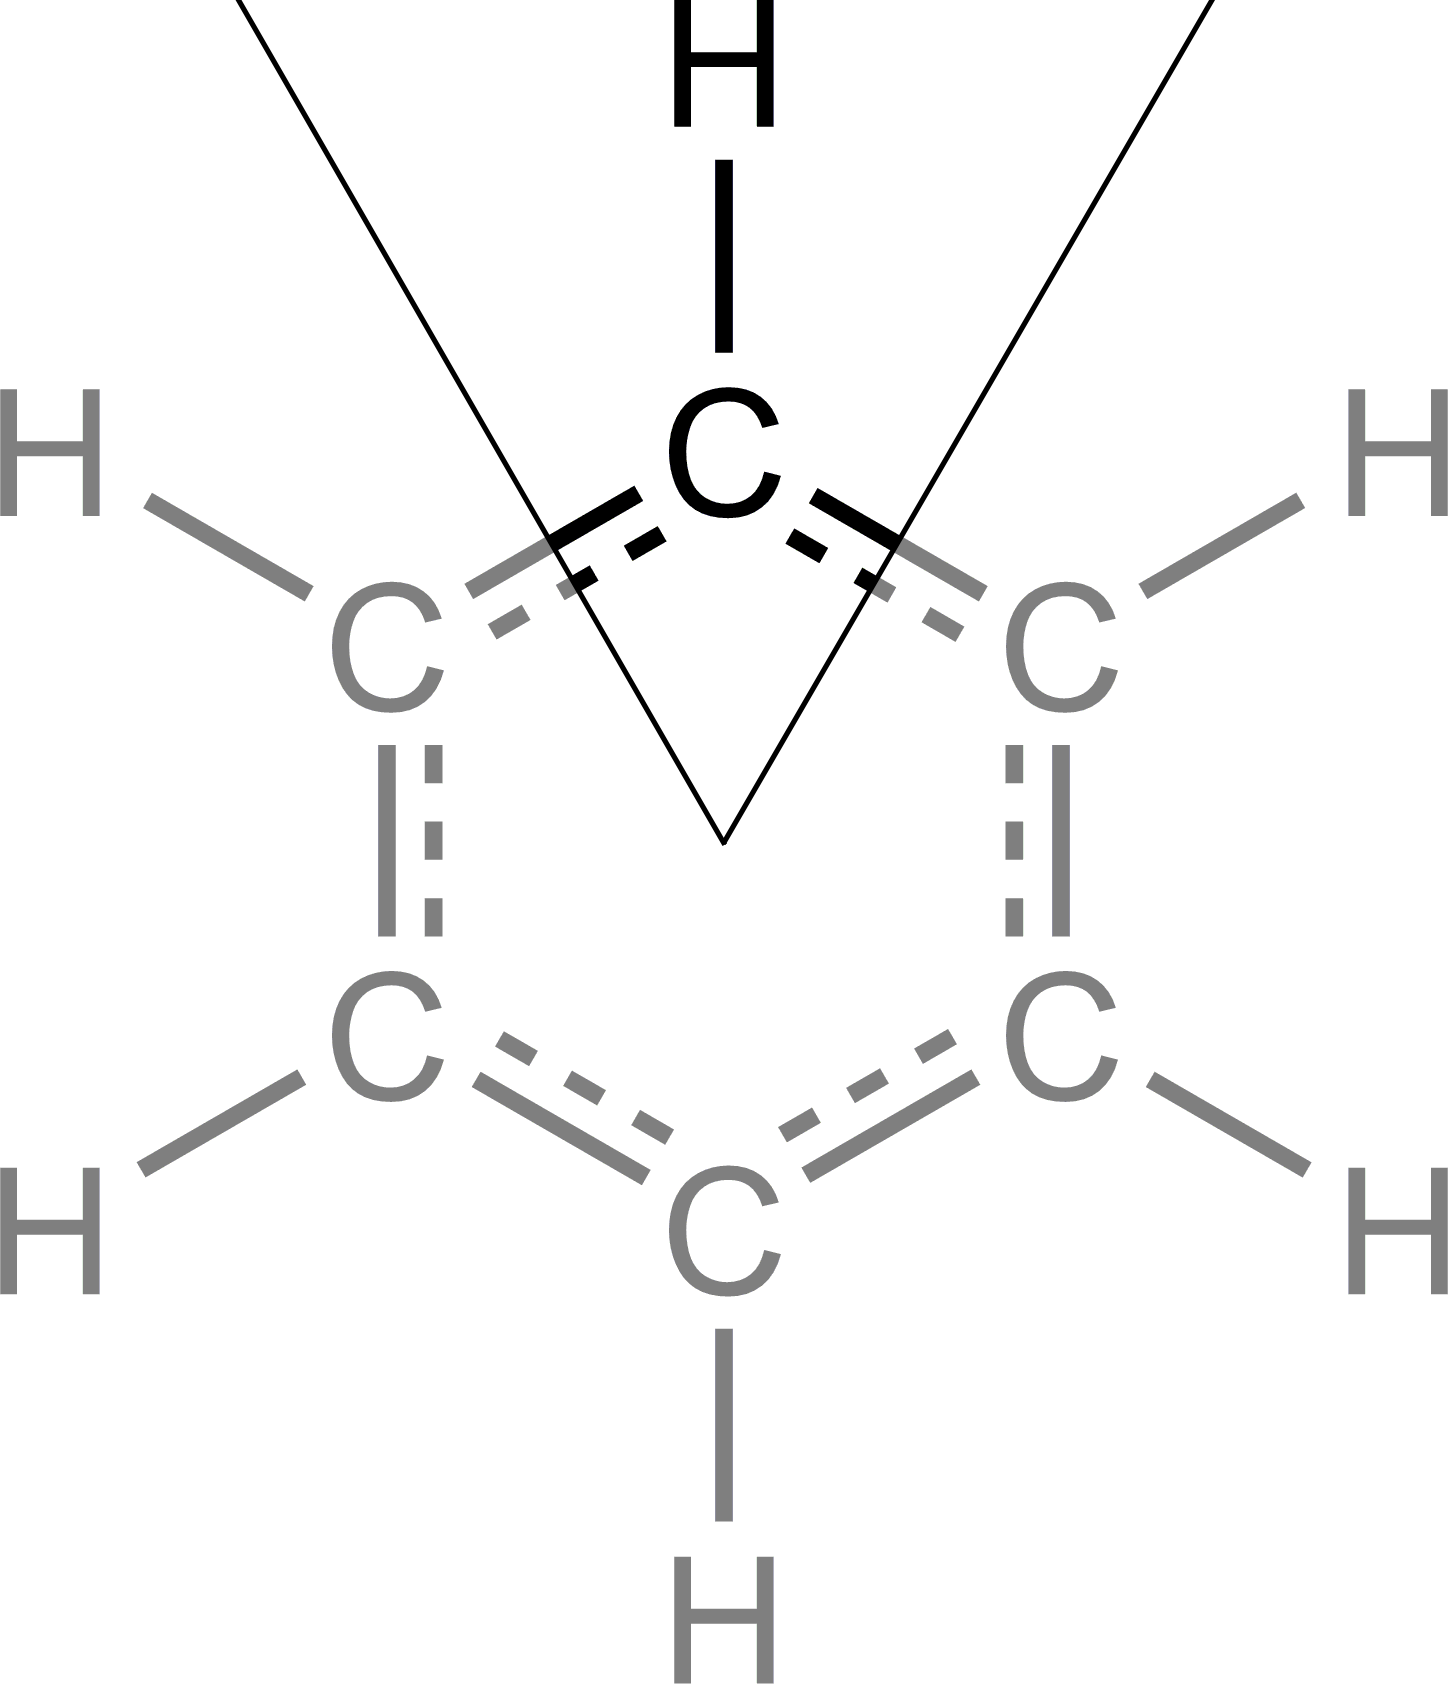
\includegraphics[scale=0.22]{Images/Benzene-1.png}} &
			\centering
			{$\xrightarrow{\mathmakebox[.85cm]{\hat{C}_6}}$} & 
			{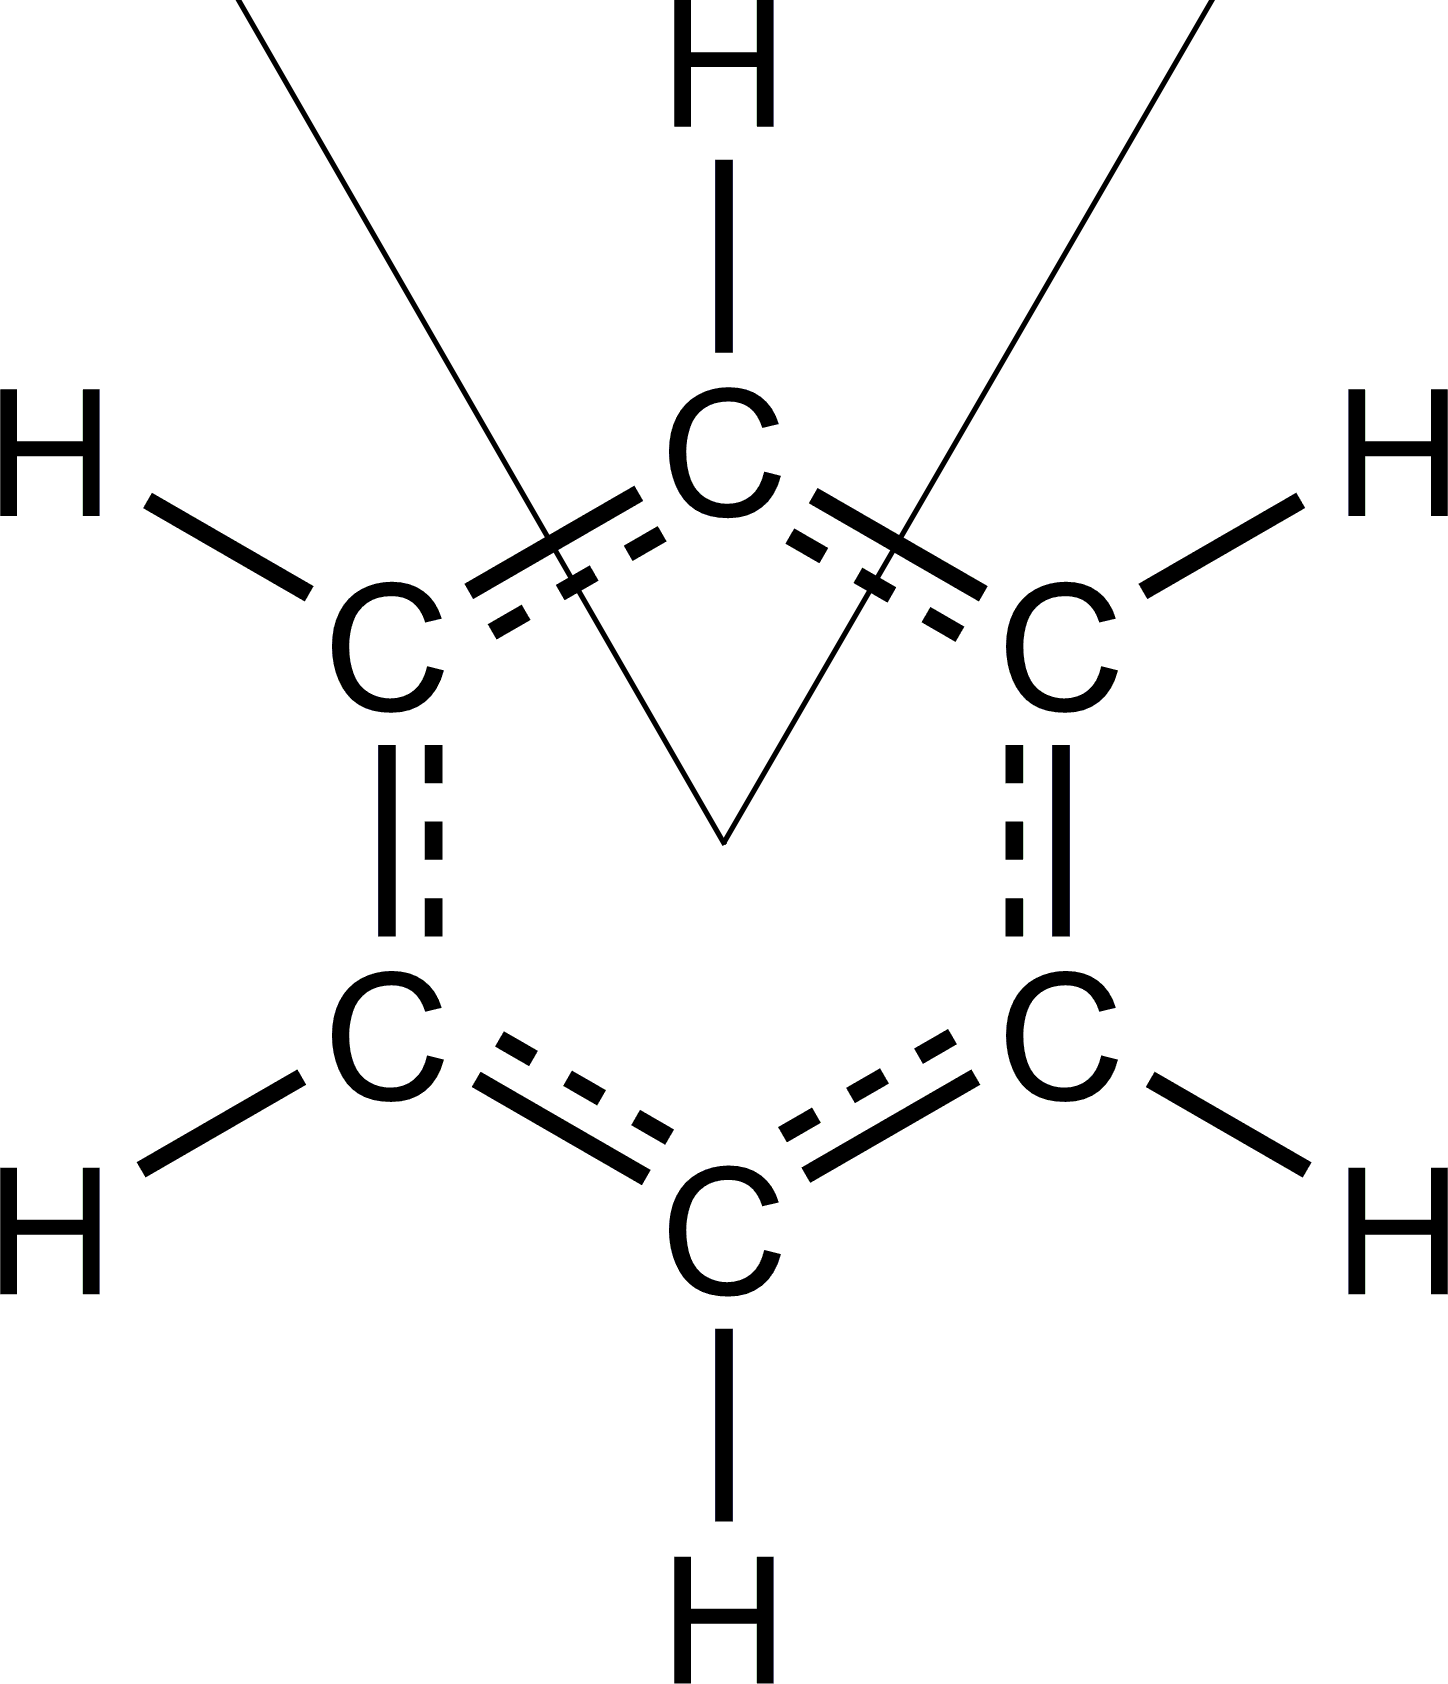
\includegraphics[scale=0.22]{Images/Benzene-2.png}}
		\end{tabular}		
	} 
	&{}
	&{	\begin{tabular}[m]{m{3.3cm}m{0.75cm}m{3.5cm}}
			{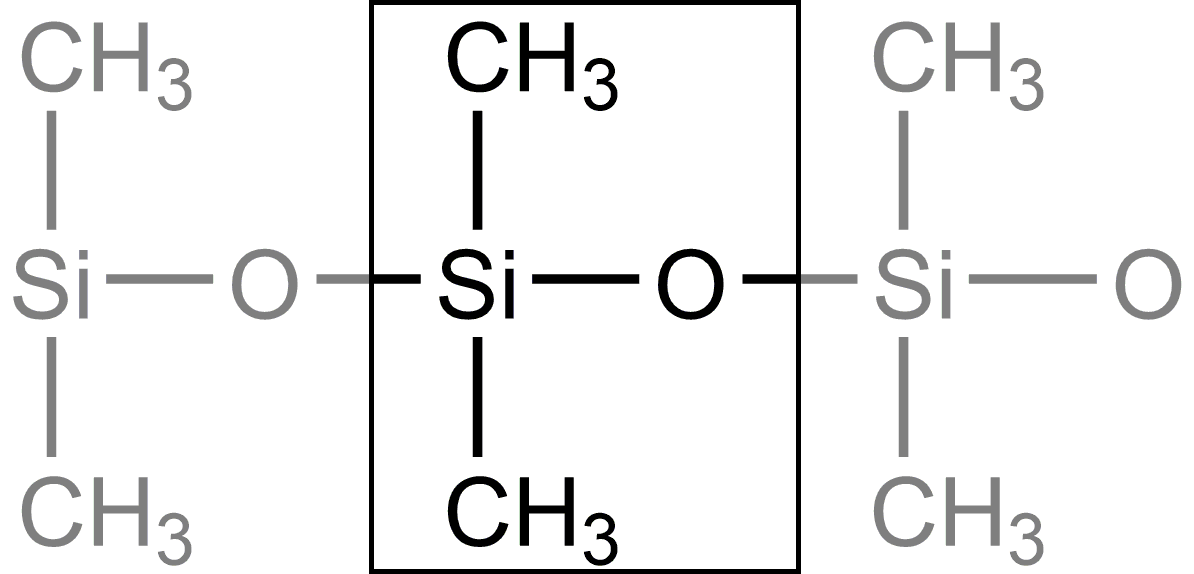
\includegraphics[scale=0.35]{Images/SiOR-1.png}} &
			{$\xrightarrow{\mathmakebox[.75cm]{\hat{T}_n}}$} & 
			{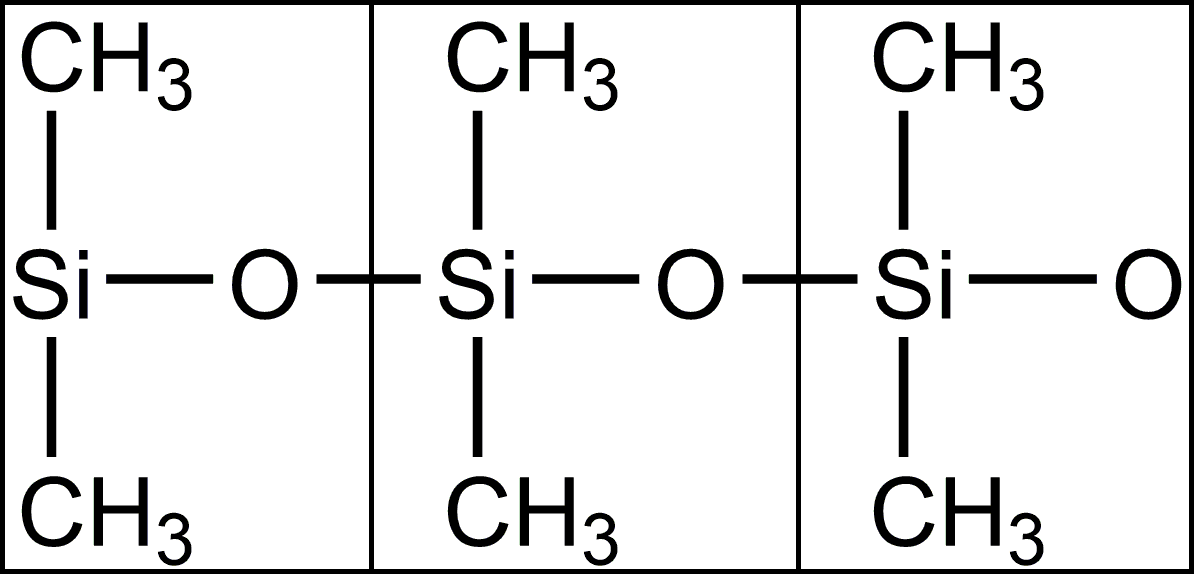
\includegraphics[scale=0.35]{Images/SiOR-2.png}}
		\end{tabular}
	}\\
		\centering (a) & &
		\centering (b)		
	\end{tabular}
	\caption[Unit cells of benzene and polydimethylsiloxane]
		{(a) C$_6$ symmetry of Benzene and (b) Translational symmetry of \ce{(SiO(CH3)2)$_n$}}	
	\label{Fig:unit cell}	
\end{figure}

\begin{figure}
\centering
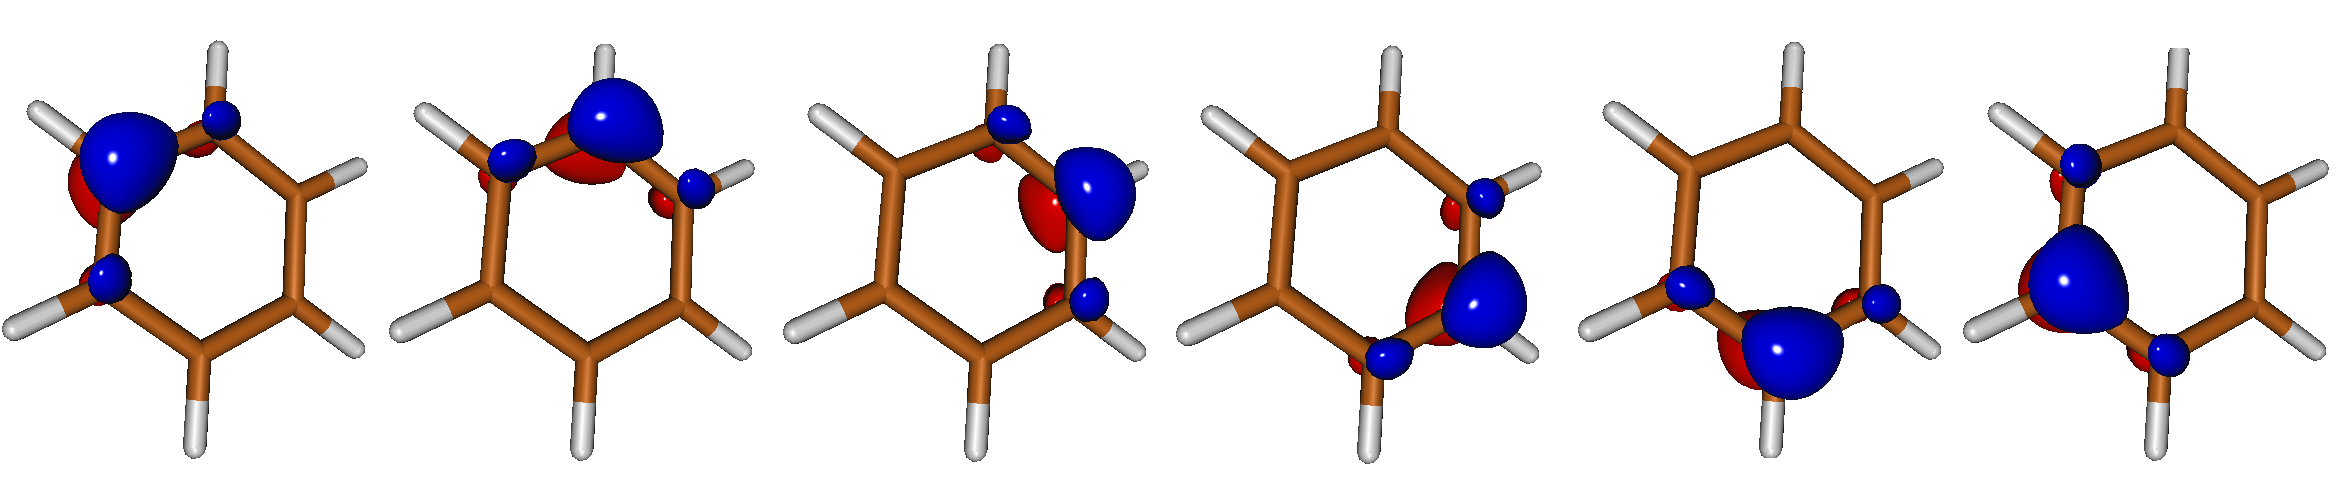
\includegraphics[scale=2]{Images/CLOBenHor.png}
\caption{Benzene CLO $\pi$ orbitals}
\label{fig:PiClo}
\end{figure}


\begin{figure}
\centering
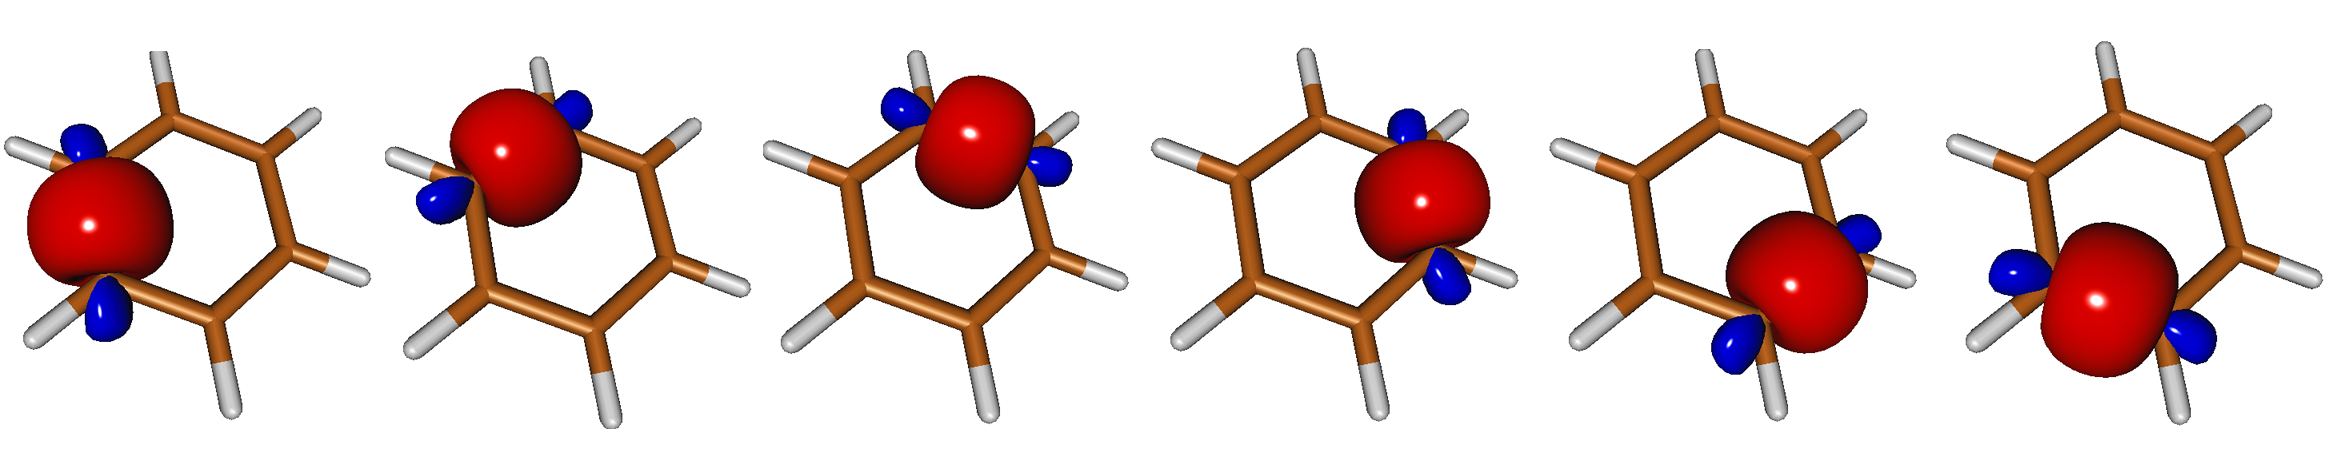
\includegraphics[scale=2]{Images/CLOBensig.png}
\caption{Benzene CLO \ce{CC} $\sigma$ orbitals}
\label{fig:SigClo}
\end{figure}

CLOs need only be constructed for the central unit cell, while orbitals on other fragments can be constructed by applying operations in $\mathcal{H}$. An additional significant advantage with CLOs is that only unique integrals, residuals, and t-amplitudes need to be calculated. For example, for a pair of occupied orbitals $i, \, j$ and an associated t-amplitude, $t^{ab}_{ij}$, one of the occupied labels, say $i$, is associated with the central unit cell, while j can reside anywhere. The t-amplitude is vanishingly small for $i, \, j$ which are far apart. The construction of the CLOs scales only with the size of the unit cell, and not the overall system (i.e. scales as $\mathcal{O}(1)$ with system size). As a result, the CLOs can, in principle, be constructed for systems of any size, including solids.

\subsubsection{Partitioning of r$^{-1}$ Potentials}
Consider the nuclear-nuclear interaction in an infinite lattice of repeating unit cells. 
\begin{equation}
E_{NN}=\frac{1}{2}\sum_{i,j} \frac{Z_i Z_j}{r_{ij}}
\label{eq:coulomb}
\end{equation}
This Coulomb interaction, which is trivial to compute in molecular systems, introduces several problems in the condensed state.  Firstly, this interaction falls with $r^{-1}$ and as a result is very slow to converge. Secondly, there is a singularity at $r=0$. Conventionally, this potential is partitioned into a long-range component and a short range component. As given in Alavi's \textit{Electronic Structure in the Condensed State} \cite{alavi}:

\begin{equation}
\frac{1}{r} =\overbrace{\frac{\erf({\frac{r}{\alpha}})}{r}}^{\text{long-range}} + \overbrace{\frac{\erfc({\frac{r}{\alpha}})}{r}}^{\text{short-range}}
\label{eq:partition}
\end{equation} 
The short-range partition contains the singularity at $r=0$ and decays rapidly for $r > \alpha$. The long-range partition approaches $r^{-1}$ for values of $r > 2\alpha $ and has a well-defined limit as $r \rightarrow 0$; 
\begin{equation}
\lim_{r \rightarrow 0} \frac{\erf({\frac{r}{\alpha}})}{r} = \frac{2}{\alpha \sqrt{\pi}}
\end{equation}

Inserting \eqref{eq:partition} into \eqref{eq:coulomb} and expressing the long-range potential as a Fourier transform yeilds the Ewald summation of $E_{NN}$\cite{Ewald} , 

\begin{equation}
E_{NN} =\underbrace{\frac{1}{2}\sum_{i,j}  \sum_T^{T_{max}} Z_i Z_j  \frac{\erfc\big(\frac{|r_{ij}-T|}{\alpha}\big)}{|r_{ij}-T|}}_{\text{short-range in r-space}} -  \underbrace{\frac{4 \pi}{2 \Omega} \sum^{k_{max}}_k |S_k|^2 \frac{e^{-k^2\alpha^2}}{k^2}}_{\text{long-range in k-space}} -\underbrace{\frac{1}{\alpha \sqrt{\pi}} \sum_i Z^2_i}_{\text{lr "self" correction}}
\end{equation}
Where T is a lattice translation, $\Omega$ is the volume of the unit cell, $S_K$ is the nuclear structure factor, and the final term removes the self ($i=j$) terms from the long-range expression. While this example is focused on the nuclear-nuclear energy, this partitioning can be used with any $\frac{1}{r}$ interaction. Care must be taken in choosing $\alpha$ such that the computational cost of computing the short and long-range components is roughly equal. Partitioning of $\frac{1}{r}$, and in particular the Fourier treatment of long-range interactions, is key to the treatment of solids. 
\label{subsubsec:Partitioning}

%%%%%%%%%%%%%%%%%%%%%%%%%%%%%%%%%%%%%%%
\section{Proposal}
The long term goal is to develop local CC methods for solid state systems. This requires two major developments: The use of symmetry in conjunction with local correlation approaches, and the use of Fourier transform techniques to deal with slowly converging long-range Coulomb interactions. This proposal aims to make progress on both issues:

\begin{description}
\item[Orbital Localization] Performing CC calculations with a basis of localized orbitals will improve computational scaling. By using CLOs we have a localized basis that also reflects the molecular symmetry of the system, allowing us to exploit both symmetry and sparsity. The construction of the CLOs scales with the size of the unit cell, and thus CLOs can be constructed for high-symmetry molecules, and in particular, solids.
\item[Improved Partitioning] By modifying the $\erf/\erfc$  partitioning scheme, we can obtain a 'clean' separation of the two potentials, allowing for accurate calculation of purely long-range contributions which can be treated via Fourier transform.
\end{description}

First, we will discuss the construction and implementation of CLOs in the context of coupled cluster calculations. Then, we will describe a modification to the $\erf $ partitioning of the long-range potential in solids. Finally, we will discuss the partitioning in terms of Gaussian integrals and t-amplitudes.


\subsection{Orbital Localization}
\subsubsection{Construction of Congruent Localized Orbitals} \label{subsec:ConstructionCLO}
We use the following matrix index notation:
\begin{align*}
&i,j \dots \rightarrow \text{Occupied MOs} & \alpha , \beta \dots \rightarrow \text{AOs} && \mu  , \nu \dots \rightarrow \text{CLOs}
\end{align*}
We represent our occupied MOs as a linear combination of AOs,
\begin{align}
\ket{i} &= \sum_{\alpha} \ket{\alpha} C_{\alpha i}
\end{align}
Where the AO coefficients, $C_{\alpha i}$, are obtained from  a starting SCF calculation. The AO overlap matrix, $\matr{S}$, and full density matrix, $\matr{D}$, are defined as usual,
\begin{align}
\matr{S}_{\alpha \beta} &= \braket{\alpha|\beta}\\
\matr{C^{\dagger}SC} &= \matr{\mathbb{I}}\\
\matr{D}_{\alpha \beta}=\matr{CC^{\dagger}}&=\sum_i \matr{C}_{\alpha i}\matr{C}_{\beta i}
\end{align}
To build the CLOs, the atoms (and their AOs) are first partitioned into subsets, with each subset associated with a particular unit cell, $\mathcal{B}_i$. To form a basis for our CLOs, we construct and diagonalize a matrix,
\begin{align}
(\matr{SDS})_{\mathcal{B}_1} \tilde{\matr{u}}^{\mathcal{B}_1} &= \matr{S}_{\mathcal{B}_1} \matr{\tilde{u}}^{\mathcal{B}_1}
\label{eq:SDSmuA}
\end{align}
Where ${\mathcal{B}_1}$ indicates that we take the block of $\matr{SDS}$ associated with one particular unit cell. Solving this eigenvalue problem gives us AO coefficients, $u^{\mathcal{B}_1}_{\alpha\mu} $,  for CLOs located on unit cell ${\mathcal{B}_1}$. CLOs on unit cells equivalent to ${\mathcal{B}_1}$ can be obtained by a simple symmetry operation (rotation, reflection, inversion),  $\hat{R}_i$ .
\begin{align}
{\mathcal{B}_i} &= \hat{R}_i {\mathcal{B}_1}
\label{eq:muCoeff}
\end{align}
This procedure [\eqref{eq:SDSmuA} and \eqref{eq:muCoeff}] is repeated for all unit cells. We now have a set of (possibly) linearly dependent CLOs which span the occupied space and are fully localized. To perform calculations using existing CC implementations, this CLO basis must meet two criteria:

\begin{enumerate}
\item If linearly independent, orbitals must be orthonormal
\item If linearly dependent, the  density matrix, $\matr{D}_{CLO}$, must be idempotent
\end{enumerate} 
For the purpose of this report, it is sufficient to show that we can build an idempotent density matrix from an arbitrary set of orbitals. First, we build
\begin{align}
\matr{x}_{ij} = \sum_\mu \matr{u}_{i \mu} \matr{u}_{j \mu} = \matr{u} \matr{u}^\dagger
\end{align}
We then take the regularized inverse of $\matr{x}$, $\matr{x}^{-\frac{1}{2}}$, and define our final CLO orbitals and overlap matrix as 
\begin{align}
\matr{\tilde{u}} &= \matr{x^{-\frac{1}{2}}} \matr{u} \label{eq:xij} \\
\matr{D}_{CLO_{\mu \nu}} &= \sum_i \matr{\tilde{u}}_{i \mu} \matr{\tilde{u}}_{i \nu}
\end{align} 
\begin{proof} $D_{CLO}$ is idempotent
\begin{align*}
\matr{D}_{CLO_{\mu \nu}} &= \sum_i \matr{\tilde{u}}_{i \mu} \matr{\tilde{u}}_{i \nu} = \matr{\tilde{u}}^\dagger \matr{\tilde{u}} && \matr{\tilde{u}} = \matr{x}^{-\frac{1}{2}}\matr{u} \\
&= \matr{u}^{\dagger} \matr{x}^{-\frac{1}{2}} \matr{x}^{- \frac{1}{2}}\matr{u} = \matr{u}^{\dagger} \matr{x}^{-1}\matr{u} \\
\matr{D}_{CLO}\matr{D}_{CLO} &= \matr{u}^{\dagger} \matr{x}^{-1}\matr{u} \matr{u}^{\dagger} \matr{x}^{-1}\matr{u}&& \matr{u} \matr{u}^{\dagger} = \matr{x} \\
&=  \matr{u}^{\dagger} \matr{x}^{-1} \matr{x} \matr{x}^{-1}\matr{u}  \\
&= \matr{u}^{\dagger} \matr{x}^{-1} \matr{u} = \matr{D}_{CLO}
\end{align*}
\end{proof}

Using the orbitals defined by the idempotent density matrix allows the constructed CLOs to be used in existing CC implementations. When performing these calculations, care must be taken as a subset of the CLOs are still linearly dependent. If the system in question is finite, we may lift this linear dependency by creating a subset of orbitals which are not congruent, but which may be localized. For solids, there is no alternative, and the linearly dependent orbitals must be used. Thankfully, the CC equations can be solved with linearly dependent orbitals without substantial changes to the algorithm. This has been tested for a small number of test cases, but further work is needed. 

\subsubsection{Using CLOs in CC calculations and Short-Range Interactions}
Congruent localized orbitals have successfully been built for benzene, cubane, ferrocene, and \ce{SF6}. Currently, a preliminary implementation of the CLOs is available in ACESII, and these orbitals can be fed into a conventional solver for the CCSD equations. This implementation needs further testing, in particular regarding the solution of the CCSD equations for a set of linearly dependent CLOs. Further improvements of the CLO implementation in ACESII will be pursued using a software tool recently developed by Mike Lecours to automatically break up molecules into congruent cells, with automatic determination of the associated symmetry groups and operators. In parallel, in collaboration with Dr. Ondrej Demel, an implementation of the CLOs will be pursued in ORCA. This implementation can then be combined with a symmetrized DLPNO-CC approach. 

\subsection{Improved Partitioning of the Long-Range Potential}
To model the long range potential, we will use a modified form of \eqref{eq:coulomb}. In particular, we multiply the long-range term of \eqref{eq:coulomb} by a smoothing function, $\theta(r)$. 
\begin{align}
f(r)&=\frac{\erf(\omega r)}{r} & \omega=\frac{1}{\alpha} \\
\theta (r;a,b)&=\frac{1}{2}\bigg(1+\erf\bigg({\frac{r-a}{b}}\bigg)\bigg)\\
V_{lr}(r) &= \theta(r) f(r)\\
V^{\text{new}}_{lr}(r) &=  \frac{1}{2} \bigg(1+\erf\bigg({\frac{r-a}{b}}\bigg)\bigg)\frac{\erf(\omega r)}{r} = \theta(r;a,b) \, V^{\text{old}}_{lr}(r) & \omega=\frac{1}{\alpha}
\end{align}
Defining $V_{lr}$ this way allows us to adjust $\theta(r)$ to tune the shape of our potential. The parameter $a$ controls when $V_{lr}$ 'switches' on, and b controls the rate of this transition. Plots of $V_{lr}$ with varying parameters are given in Figure \ref{AdjustingVlr}. \medskip \newline

\begin{figure}[H]
	\begin{tabular}[m]{m{0.33\textwidth}m{0.33\textwidth}m{0.33\textwidth}}
		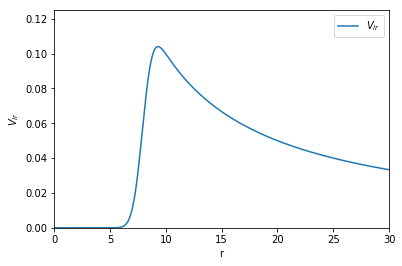
\includegraphics[width=0.33\textwidth]{Images/Vlra8b1.png}&
		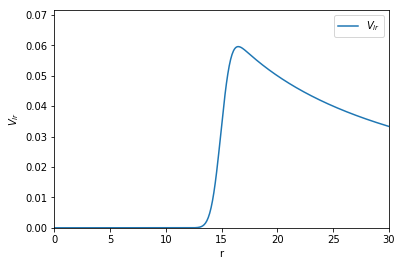
\includegraphics[width=0.33\textwidth]{Images/Vlra15b1.png}&
		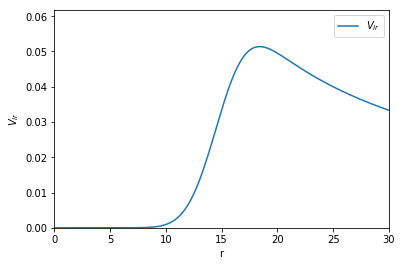
\includegraphics[width=0.33\textwidth]{Images/Vlra15b3.png} \\
		\centering $V_{lr}(r,a=8, b=1)$&
		\centering $V_{lr}(r,a=15, b=1)$&
		\centering $V_{lr}(r,a=15, b=3)$
	\end{tabular}
	\caption{Fine-tuning $V_{lr}$ by adjusting $a, b$}
	\label{AdjustingVlr}
\end{figure}

As previously stated in \S \ref{subsubsec:Partitioning}, integrals over $V_{lr}(r)$ converge slowly due to the $r^{-1}$ decay of the potential. Fortunately, due to the uncertainty principle, functions with large spatial dispersion have compact counterparts in momentum space (Figure \ref{TransformVlr}). Therefore, integrals over the Fourier transform of $V_{lr}(r)$, will quickly converge. For simplicity, we define 
\begin{equation}
\hat{V}_{lr}(k) \equiv \mathcal{F}[V_{lr}(r)](k) 
\end{equation}

\begin{figure}[h]
	\begin{tabular}[m]{m{0.5\textwidth}m{0.5\textwidth}}
		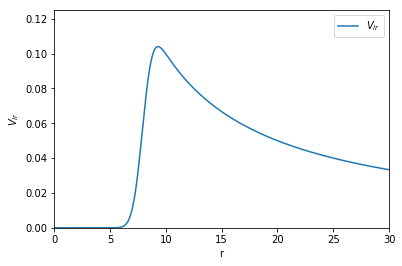
\includegraphics[width=0.5\textwidth]{Images/Vlra8b1.png} & 
		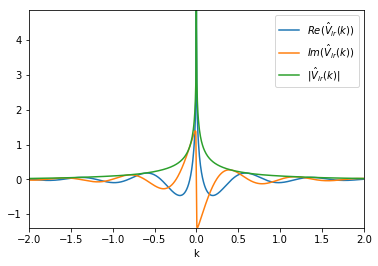
\includegraphics[width=0.5\textwidth]{Images/FVlr.png}\\
		\centering$V_{lr}(r)$, spread out in r-domain & 
		\centering$\hat{V}_{lr}(k)$, concentrated in k-domain
	\end{tabular}
	\caption{$V_{lr}(r)$ and $\hat{V}_{lr}(k)$}	
	\label{TransformVlr}
\end{figure} 
 
Before we can perform meaningful calculations with $\hat{V}_{lr}$, we must deal with the singularity at $k=0$. This singularity is due to the $k^{-2}$ dependence of $\hat{V}_{lr}$. If we evaluate our integrals using spherical coordinates, the $k^2$ volume element of the integral will remove this singularity, as shown in Figure \ref{FVLR}. 

\begin{figure}[h]
	\begin{tabular}[m]{m{0.5\textwidth}m{0.5\textwidth}}
		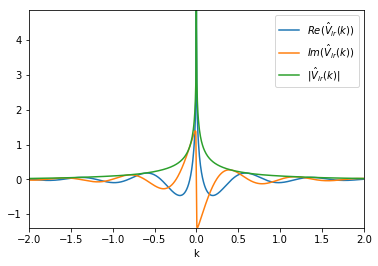
\includegraphics[width=0.5\textwidth]{Images/FVlr.png}&
		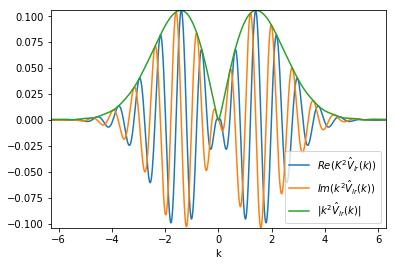
\includegraphics[width=0.5\textwidth]{Images/FVlrk2.png} \\
		\centering $\hat{V}_{lr}(K)$ & 
		\centering $k^2 \hat{V}_{lr}(k)$
	\end{tabular}
	\caption{Removing the $k=0$ singularity using spherical coordinates}
	\label{FVLR}
\end{figure}

By calculating $ \hat{V}_{lr}(k, \theta, \phi)$ via fast Fourier transform (FFT), it is possible to calculate long-range Coulomb integrals of the form
\begin{equation}
\braket{pq|\, \frac{1}{r} \,|rs}_{lr} = \braket{pq | \vec{k}} \hat{V}_{lr}(\vec{k},\theta,\phi) \braket{\vec{k}|rs}
\end{equation}

where $p, q, r,$ and $s$ are regular Gaussian AO functions calculated analytically.
A recurrence relation for analytically calculating the Fourier transform of Gaussian products previously developed by Sun et al. \cite{sun} is given in supplementary \ref{SUP:pyscf}. The overall integral can then be evaluated numerically via Gauss-Lebedev quadrature. The accurate calculation of the 2e integrands using resolution of the identity is a non-trivial issue that will be investigated throughout the project. 

%%%%%%%%%%%%%%%%%%%%%%%%%%%%%%%%%%%%%%%
\subsection{Partitioning contributions in CC calculations}

In the evaluation of the correlation energy for solids, the use of Fourier technique to obtain convergence is crucial, and an efficient way to pursue this is as follows. Fock matrix contributions from the long-range potential can be calculated via FFT and Gauss-Levbedev quadrature. This, however, comes at a cost: because we have modified the long-range potential (and in turn the partitioning) there is no analytical formula for calculating short-range potential, or its contributions to the Fock matrix. Fortunately, the following relation holds true:
\begin{align}
V_{\text{total}} &= V_{sr} + V_{lr}\\
V_{sr} &= V_{\text{total}} - V_{lr}
\end{align}
So we can obtain the short-range potential by subtracting the long-range potential from the total.  The t-amplitudes are separated into two contributions; for a given $t^{ab}_{ij}$: 
\begin{align}
{}^{\text{total}}\!t^{ab}_{ij} &= {}^{sr}\!t^{ab}_{ij} + {}^{lr}\!t^{ab}_{ij}
\end{align}
At this point we are free to chose the level of theory at which each contribution is calculated. The short-range interactions are strong and will be treated with the CLO implementation of DLPNO-CC to ensure accuracy and circumvent the harsh scaling of conventional CCSD. The long-range interactions are weaker and will be treated with MP2. Once the t-amplitudes are found, the CC energy is readily available: 
\begin{align}
E_{CC}=V_{\text{total}} \cdot T^{CC}_{sr} + V_{\text{total}} \cdot T^{MP2}_{lr} \label{Aixi}
\end{align}
Previous work by the members of the Nooijen group has shown that \eqref{Aixi} does not hold for systems in which the long and short range potentials are conventionally partitioned. If this approach works, and the new partitioning successfully isolates short and long-range contributions, one can implement an efficient MP2 treatment of the long-range interactions.  As a result, it will be possible to computationally study chemical phenomenon which are purely long or short range in nature (or,  consequently, investigate toy systems in which either interaction is intentionally excluded). In the event that our improved partitioning is not sufficiently accurate, the the conventional partitioning can be used, leading to efficient 3-center resolution of the identity representations of two electron integrals. However, the long-range interactions will likely have to be treated at the CC level. 
\section{Summary}
CLOs have been successfully constructed for finite molecular systems such as \ce{SF6} and benzene. If CC calculations using CLOs are successful, a modified DLPNO-CC method using CLOs is to be implemented for use in ORCA in collaboration with Dr. Ondrej Demel. Efficient algorithms developed using CLOs can reduce computational complexity by exploiting both molecular symmetry and orbital localization. Energy contributions with a sharp falloff in $r$ can be treated via an accuracy hierarchy, as in DLPNO-CC. Contruction of the CLOs scales independently of system size, and as such can be generated for solid state systems. In the solid state, the CLOs provide a convenient basis for calculation of short-range interactions. A modified partitioning of the short and long range potentials is being investigated. If successful, an efficient DLPNO-CC implementation for solids in which long-range interactions are calculated via MP2 \eqref{Aixi} will be investigated and tested. If unsuccessful, conventional methods to calculate long range interactions may be used at the price of computational efficiency. 

%%%%%%%%%%%%%%%%%%%%%%%%%%%%%%%%%%%%%%%
\section{Supplementary}
\subsection{Analytical Fourier transform of Gaussian products}
Let $\mu(r)$ and $\nu(r)$ be Gaussian AO functions, the Fourier transform of their product can be separated into three Cartesian integrals, ($\matr{I}^{(x,y,z)}_{m,n}$). These integrals can in turn be evaluated using a recurrence relation. This relation was published by Sun et al. \cite{sun} and is implemented in the PYSCF package.

\begin{align*}
\mathcal{F}[\mu^* \nu]&=\int e^{-i \matr{G} \cdot \matr{r}} \mu^{*}(\matr{r}) \nu(\matr{r}) d\matr{r} = C_{\mu} C_{\nu} \matr{I}^x_{m_x, n_x} \matr{I}^y_{m_y, n_y} \matr{I}^z_{m_z, n_z} & m_i, n_i \in \mathbb{Z} \\
I^{x}_{m_x, n_x} &= \int e^{-i \matr{G_x} x} (x-r_{x \mu})^{m_x} e^{- \alpha_{\mu} (x-r_{x \mu})^2} (x-r_{x \nu})^{n_x} e^{-\alpha_{\nu} (x-r_{x\mu})^2} dx
\end{align*}

Each cartesian component is then evaluated recursively:

\begin{align*}
I^{x}_{m_x, n_x} &= I^{x}_{m_x+1, n_x-1} + (r_{x\mu} - r_{x\nu}) I^{x}_{m_x, n_x-1} \\
I^{x}_{m_x, 0} &= \frac{m_x -1}{2(\alpha_{\mu} + \alpha_{\nu})} I^{x}_{m_x-2, 0} - \bigg(r_{x \mu} - X_{\mu \nu} + \frac{i G_x}{2(\alpha_{\mu} + \alpha_{\nu})}\bigg) I^x_{m_x -1, 0}\\
I^{x}_{1, 0} &= -\bigg(r_{x \mu} - X_{\mu \nu} + \frac{i G_x}{2(\alpha_{\mu} + \alpha_{\nu})}\bigg) I^{x}_{0, 0}\\
I^{x}_{0, 0} & = \sqrt{\frac{\pi}{\alpha_{\mu} + \alpha_{\nu}}} e^{- \frac{\alpha{_\mu} \alpha_{\nu}}{\alpha_{\mu} + \alpha{_nu}} (r_{x \mu} - r_{x \nu})^2} e^{- \frac{G^2_x}{4(\alpha_{\mu} + \alpha_{\nu})}} e^{-iG_xX_{\mu \nu}}\\
X_{\mu \nu} &= \frac{\alpha_{\mu}r_{x\mu}+\alpha_{\nu} r_{x\nu}}{\alpha_{\mu} + \alpha_{\nu}}
\end{align*}
\label{SUP:pyscf}
\bibliographystyle{unsrt}
\bibliography{794}
\end{document}



